\documentclass[table,xcolor=dvipsnames,professionalfonts]{beamer}
\usepackage{xcolor}
\usepackage{booktabs}
\usepackage{graphicx}
\usepackage[percent]{overpic}
\usepackage{tikz}
\usepackage{feynmp}
\usepackage{xspace}
\usepackage{slashed}
%\usepackage[utopia]{mathdesign}
%\usepackage[charter]{mathdesign}
\usepackage[UKenglish]{babel}
\usepackage[utf8]{inputenc}
%\usepackage{lmodern}
\setbeamertemplate{navigation symbols}{}
\usepackage{appendixnumberbeamer}
%\usepackage{hepparticles}
%\usepackage{hepnicenames}
\usepackage{hepunits}
%\usepackage{bbm}

\ifpdf
\usepackage{epstopdf}
\usepackage[protrusion=true,expansion=true,tracking]{microtype}
%\DeclareGraphicsRule{*}{mps}{*}{}
\fi

\usepackage{listings}
\usepackage[framemethod=tikz]{mdframed}
\lstloadlanguages{C++}
\makeatletter
\newcommand{\srcsize}{\@setfontsize{\srcsize}{5pt}{5pt}}
\makeatother

\usepackage{fontspec}
\setmainfont{Times New Roman}[]
%\setsansfont{FrontPagePro}[Scale=MatchLowercase]
%\setmonofont{PragmataPro}[Scale=MatchLowercase]

\usetheme{Rochester}
%\usecolortheme{beaver}
\usecolortheme[named=NavyBlue]{structure}
\setbeamercolor{section in toc}{fg=black,bg=white}
%\setbeamercolor{alerted text}{fg=blue}
\setbeamercolor{structure}{fg=blue!80!black}
\setbeamercolor*{palette primary}{fg=black,bg=gray!30!white}
\setbeamercolor*{palette secondary}{fg=black,bg=gray!15!white}
\setbeamercolor*{palette tertiary}{bg=blue!80!black,fg=gray!10!white}
\setbeamercolor*{palette quaternary}{fg=blue,bg=gray!5!white}
\setbeamercolor*{sidebar}{fg=blue,bg=gray!15!white}
\setbeamercolor*{palette sidebar primary}{fg=blue!10!black}
\setbeamercolor*{palette sidebar secondary}{fg=white}
\setbeamercolor*{palette sidebar tertiary}{fg=blue!50!black}
\setbeamercolor*{palette sidebar quaternary}{fg=gray!10!white}
\setbeamercolor{titlelike}{parent=palette primary,fg=blue,bg=white}
\setbeamercolor{frametitle}{fg=white,bg=blue!80!black}
\setbeamercolor{frametitle right}{bg=gray!60!white}
\setbeamercolor*{separation line}{}
\setbeamercolor*{fine separation line}{}
\useinnertheme{rectangles}
\useoutertheme{infolines}
\usefonttheme[onlymath]{serif}
%\usefonttheme{professionalfonts}

%\loadgraphics{logo-pi-bunt3,lhcb-logo,unisiegel-gray}

% https://tex.stackexchange.com/a/98205
\newsavebox{\unilogo} \newsavebox{\pilogo} \newsavebox{\lhcblogo}
\IfFileExists{../cern-logo-gray.eps}{\sbox{\unilogo}{\includegraphics[height=1.2cm]{../cern-logo-gray.eps}} }{\sbox{\unilogo}{\includegraphics[height=1.2cm]{cern-logo-gray.eps}}}
\IfFileExists{../cern-logo.eps}{     \sbox{\pilogo}{
\includegraphics[height=0.75cm]{../cern-logo.eps}}      }{\sbox{\pilogo}{
\includegraphics[height=0.75cm]{cern-logo.eps}}     }
\IfFileExists{../lhcb-logo.eps}{\sbox{\lhcblogo}{
\includegraphics[height=0.75cm]{../lhcb-logo.eps}}}{\sbox{\lhcblogo}{
\includegraphics[height=0.75cm]{lhcb-logo.eps}}}

\setbeamertemplate{footline}
{
  \leavevmode%
  \hbox{%
    \begin{beamercolorbox}[wd=.333333\paperwidth,ht=2.25ex,dp=1ex,left]{author in head/foot}%
      \usebeamerfont{author in head/foot}\vtop{\vskip-2.25ex\hbox{\resizebox{!}{3.25ex}{\usebox{\pilogo}}}}%
      \hfill \insertshortauthor~~(\insertshortinstitute) \hfill%
    \end{beamercolorbox}%
    \begin{beamercolorbox}[wd=.333333\paperwidth,ht=2.25ex,dp=1ex,center]{title in head/foot}%
      \usebeamerfont{title in head/foot}\insertshorttitle%
    \end{beamercolorbox}%
    \begin{beamercolorbox}[wd=.333333\paperwidth,ht=2.25ex,dp=1ex,right]{date in head/foot}%
      \usebeamerfont{date in head/foot}\insertshortdate{}\hspace*{2em}%
      \insertframenumber{} / \inserttotalframenumber\hspace*{2ex} \vtop{\vskip-2.25ex\hbox{\resizebox{!}{3.25ex}{\usebox{\lhcblogo}}}}%
    \end{beamercolorbox}%
  }%
  \vskip0pt%
}

\setbeamertemplate{frametitle}
{
  \ifbeamercolorempty[bg]{frametitle}{}{\nointerlineskip}%
  \leavevmode%
  \vskip-2pt\hbox{%
    \begin{beamercolorbox}[wd=\paperwidth,left]{frametitle}%
      \usebeamerfont{frametitle}%
      \vskip.125ex%
      \hbox{\vtop{\raisebox{-1ex}[1ex][1ex]{\makebox[0pt][l]{\usebox{\unilogo}}}%
      \hspace{1em}\strut\insertframetitle\strut}\par%
      {%
        \ifx\insertframesubtitle\@empty%
        \else%
        {\usebeamerfont{framesubtitle}\usebeamercolor[fg]{framesubtitle}\insertframesubtitle\strut\par}%
        \fi
      }}%
    \end{beamercolorbox}%
  }%
}


\definecolor{bandgreen}{rgb}{0.3,0.8,0.2}
\newcommand{\FIXME}{{\color{red}FIXME}}
\newcommand{\arxiv}[1]{{\color{gray}\tiny$[$\href{http://arxiv.org/abs/#1}{arXiv:#1}$]$}}
\newcommand{\jref}[2]{{\color{gray}\tiny$[$\href{#2}{#1}$]$}}
\newcommand{\myhref}[2]{\href{#1}{\footnotesize{\textcolor{blue}{\texttt{#2}}}}}


\author[Paul Seyfert]{Paul Seyfert\newline on behalf of the LHCb collaboration}
\institute[CERN]{CERN}
\date[15th September 2017]{VERTEX 2017}
\title[LHCb upgrade]{Tracking, Vertexing and data handling strategy for the LHCb upgrade}


\begin{document}
\maketitle

\begin{frame}
  \frametitle{scope I}

  \begin{columns}
    \begin{column}{.55\textwidth}
        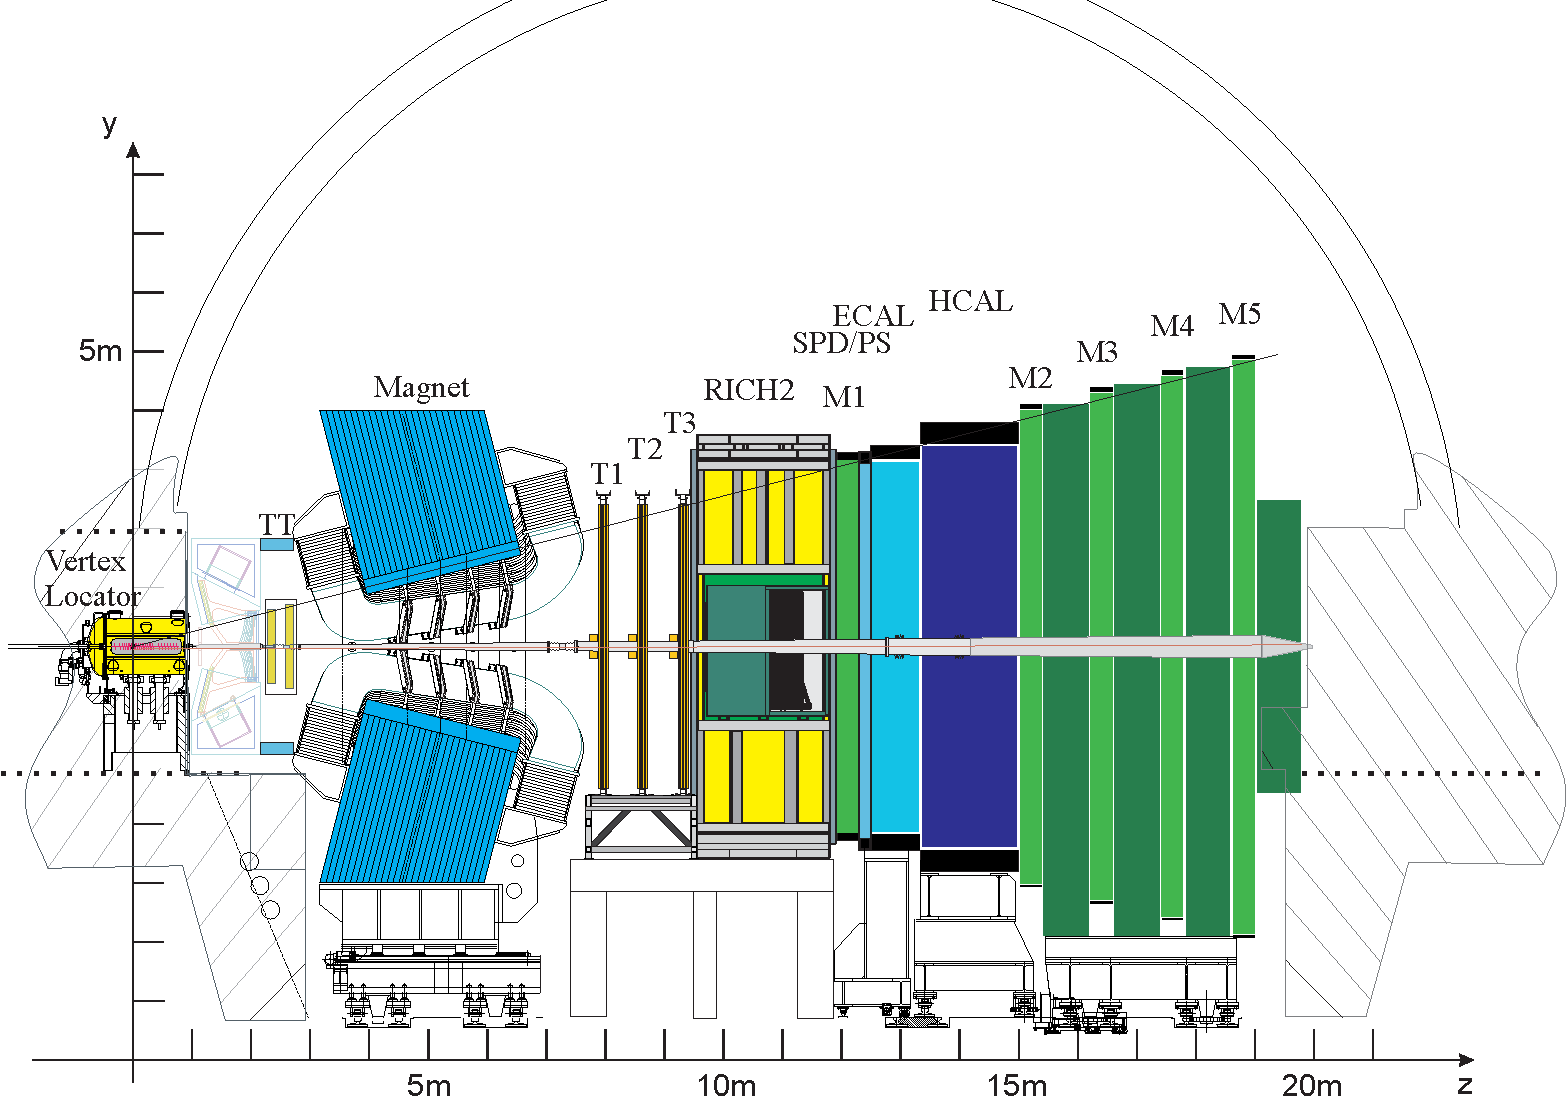
\includegraphics[width=\textwidth,trim=0 0 0 50,clip]{LHCb-reoptimized-y.pdf}

        {\myhref{http://dx.doi.org/10.1142/S0217751X15300227}{LHCb-DP-2014-002}}
    \end{column}
    \begin{column}{.45\textwidth}
      \begin{itemize}
        \item Fully equipped forward detector at the LHC
        \item Approaching 400 papers
        \item exceeding our own expectations:
          \begin{itemize}
              \item online calibration and alignment
                \newline \myhref{http://dx.doi.org/10.1016/j.nima.2016.06.050}{j.nima.2016.06.050}
              \item exceeding design pile-up
          \end{itemize}
      \end{itemize}
    \end{column}
    \end{columns}
    \end{frame}

    \begin{frame}
      \frametitle{scope II}
      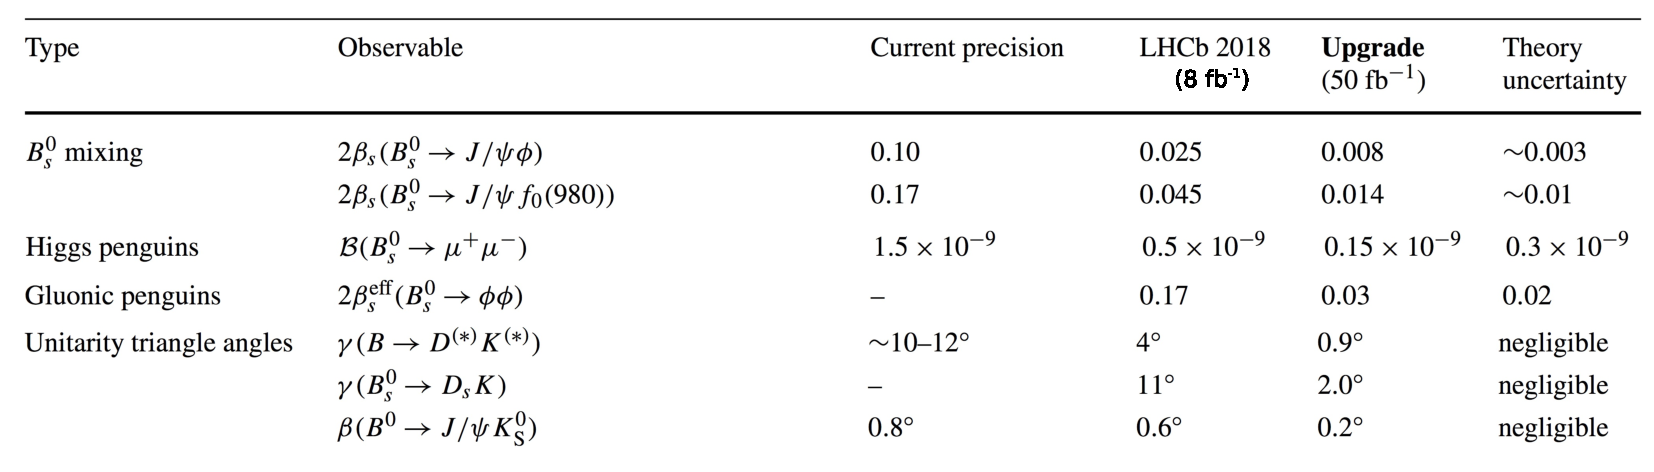
\includegraphics[width=\textwidth]{./alessiotable.pdf}

      \myhref{https://doi.org/10.1140/epjc/s10052-013-2373-2}{Eur. Phys. Journal C (2013) 73:2373}

      \begin{itemize}
          \item By 2018 important analyses will still be statistically limited
          \item Theoretical uncertainty smaller than experimental
          \item[$\rightarrow$] Significantly more statistics needed
          \item[$\Rightarrow$] Go to higher luminosity
            \newline ($\mathcal{L}=2\times10^{33}\mathrm{cm}^{-2}\mathrm{s}^{-1} \Rightarrow \nu\sim 7.6$)
            \newline \myhref{https://cds.cern.ch/record/1670985?ln=en}{LHCb-PUB-2014-027}
      \end{itemize}
    \end{frame}


    \begin{frame}
      \frametitle{Upgrade of the tracking system}
      \begin{columns}
        \begin{column}{.7\textwidth}
          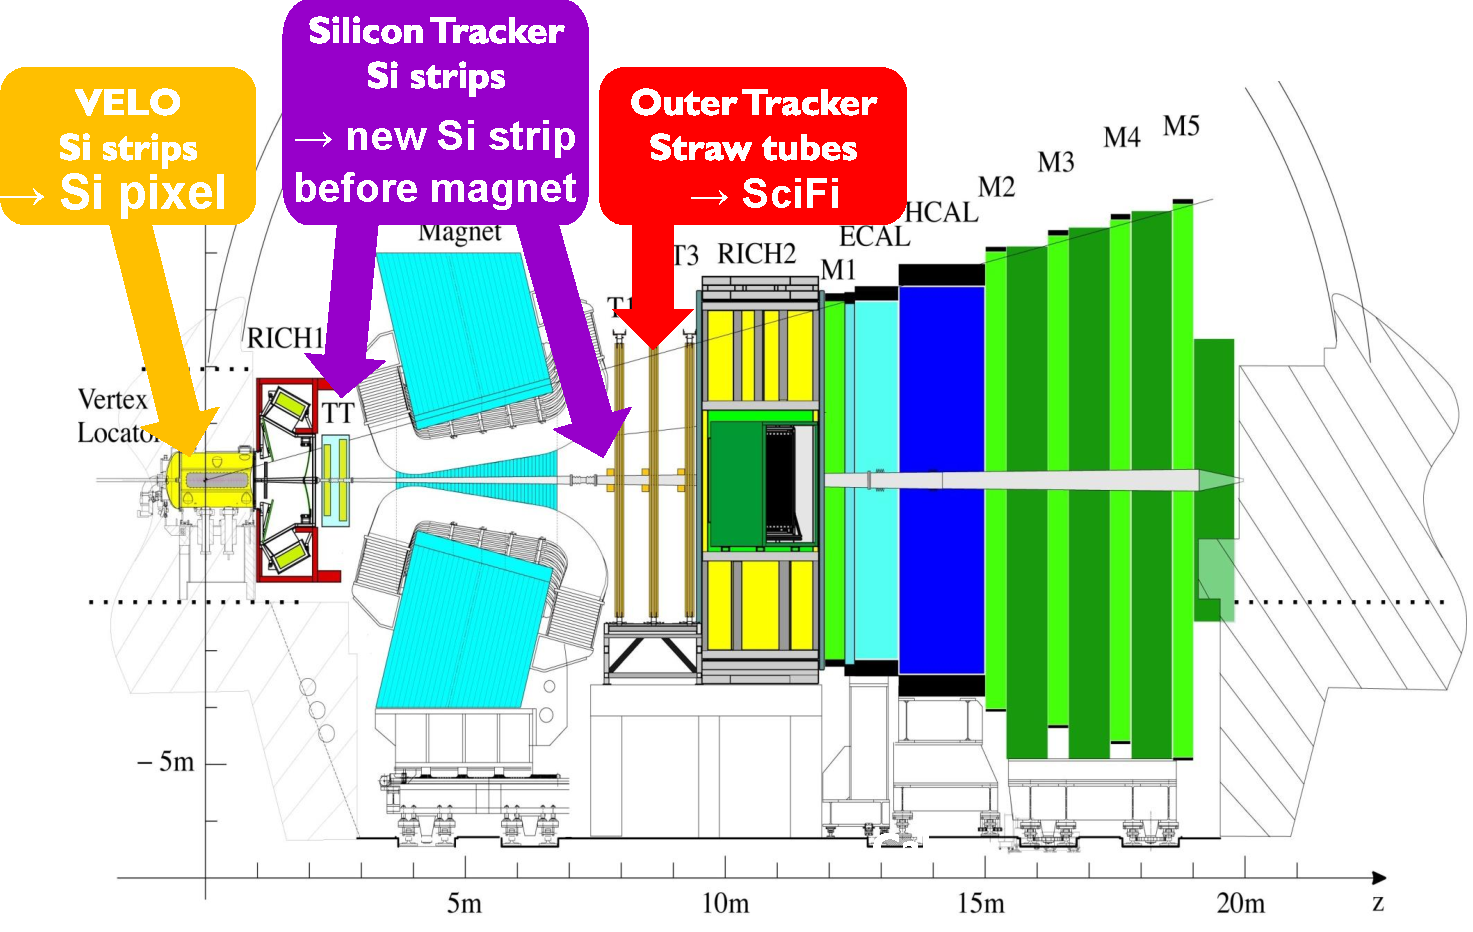
\includegraphics[width=\textwidth]{./LHCb2.pdf}
        \end{column}
        \begin{column}{.3\textwidth}
            \begin{itemize}
              \item Vertex pixel detector
                \newline see talk by Edgar Lemos Cid
              \item silicon strip detector
                \newline see talk by Marco Petruzzo
              \item scintilating fiber tracker
            \end{itemize}
          \end{column}
        \end{columns}
        \begin{columns}
        \begin{column}{.3\textwidth}
          \begin{block}{$\sigma_z$ (vertex)}
            $<\unit{90}{\micro\meter}$\newline \small{(more than 20 tracks)}
            $<\unit{50}{\micro\meter}$\newline \small{(more than 50 tracks)}
          \end{block}
          \end{column}
        \begin{column}{.3\textwidth}
          \begin{block}{$\sigma_t$ (decay)}
            $<\unit{45}{\femto\second}$
          \end{block}
          \end{column}
        \begin{column}{.3\textwidth}
          \begin{block}{$\sigma_p/p$}
            $<0.5\,\%$
          \end{block}
          \end{column}
        \end{columns}
      \end{frame}

\begin{frame}
  \frametitle{removal of hardware trigger I}
  \begin{columns}
  \begin{column}{.6\textwidth}
    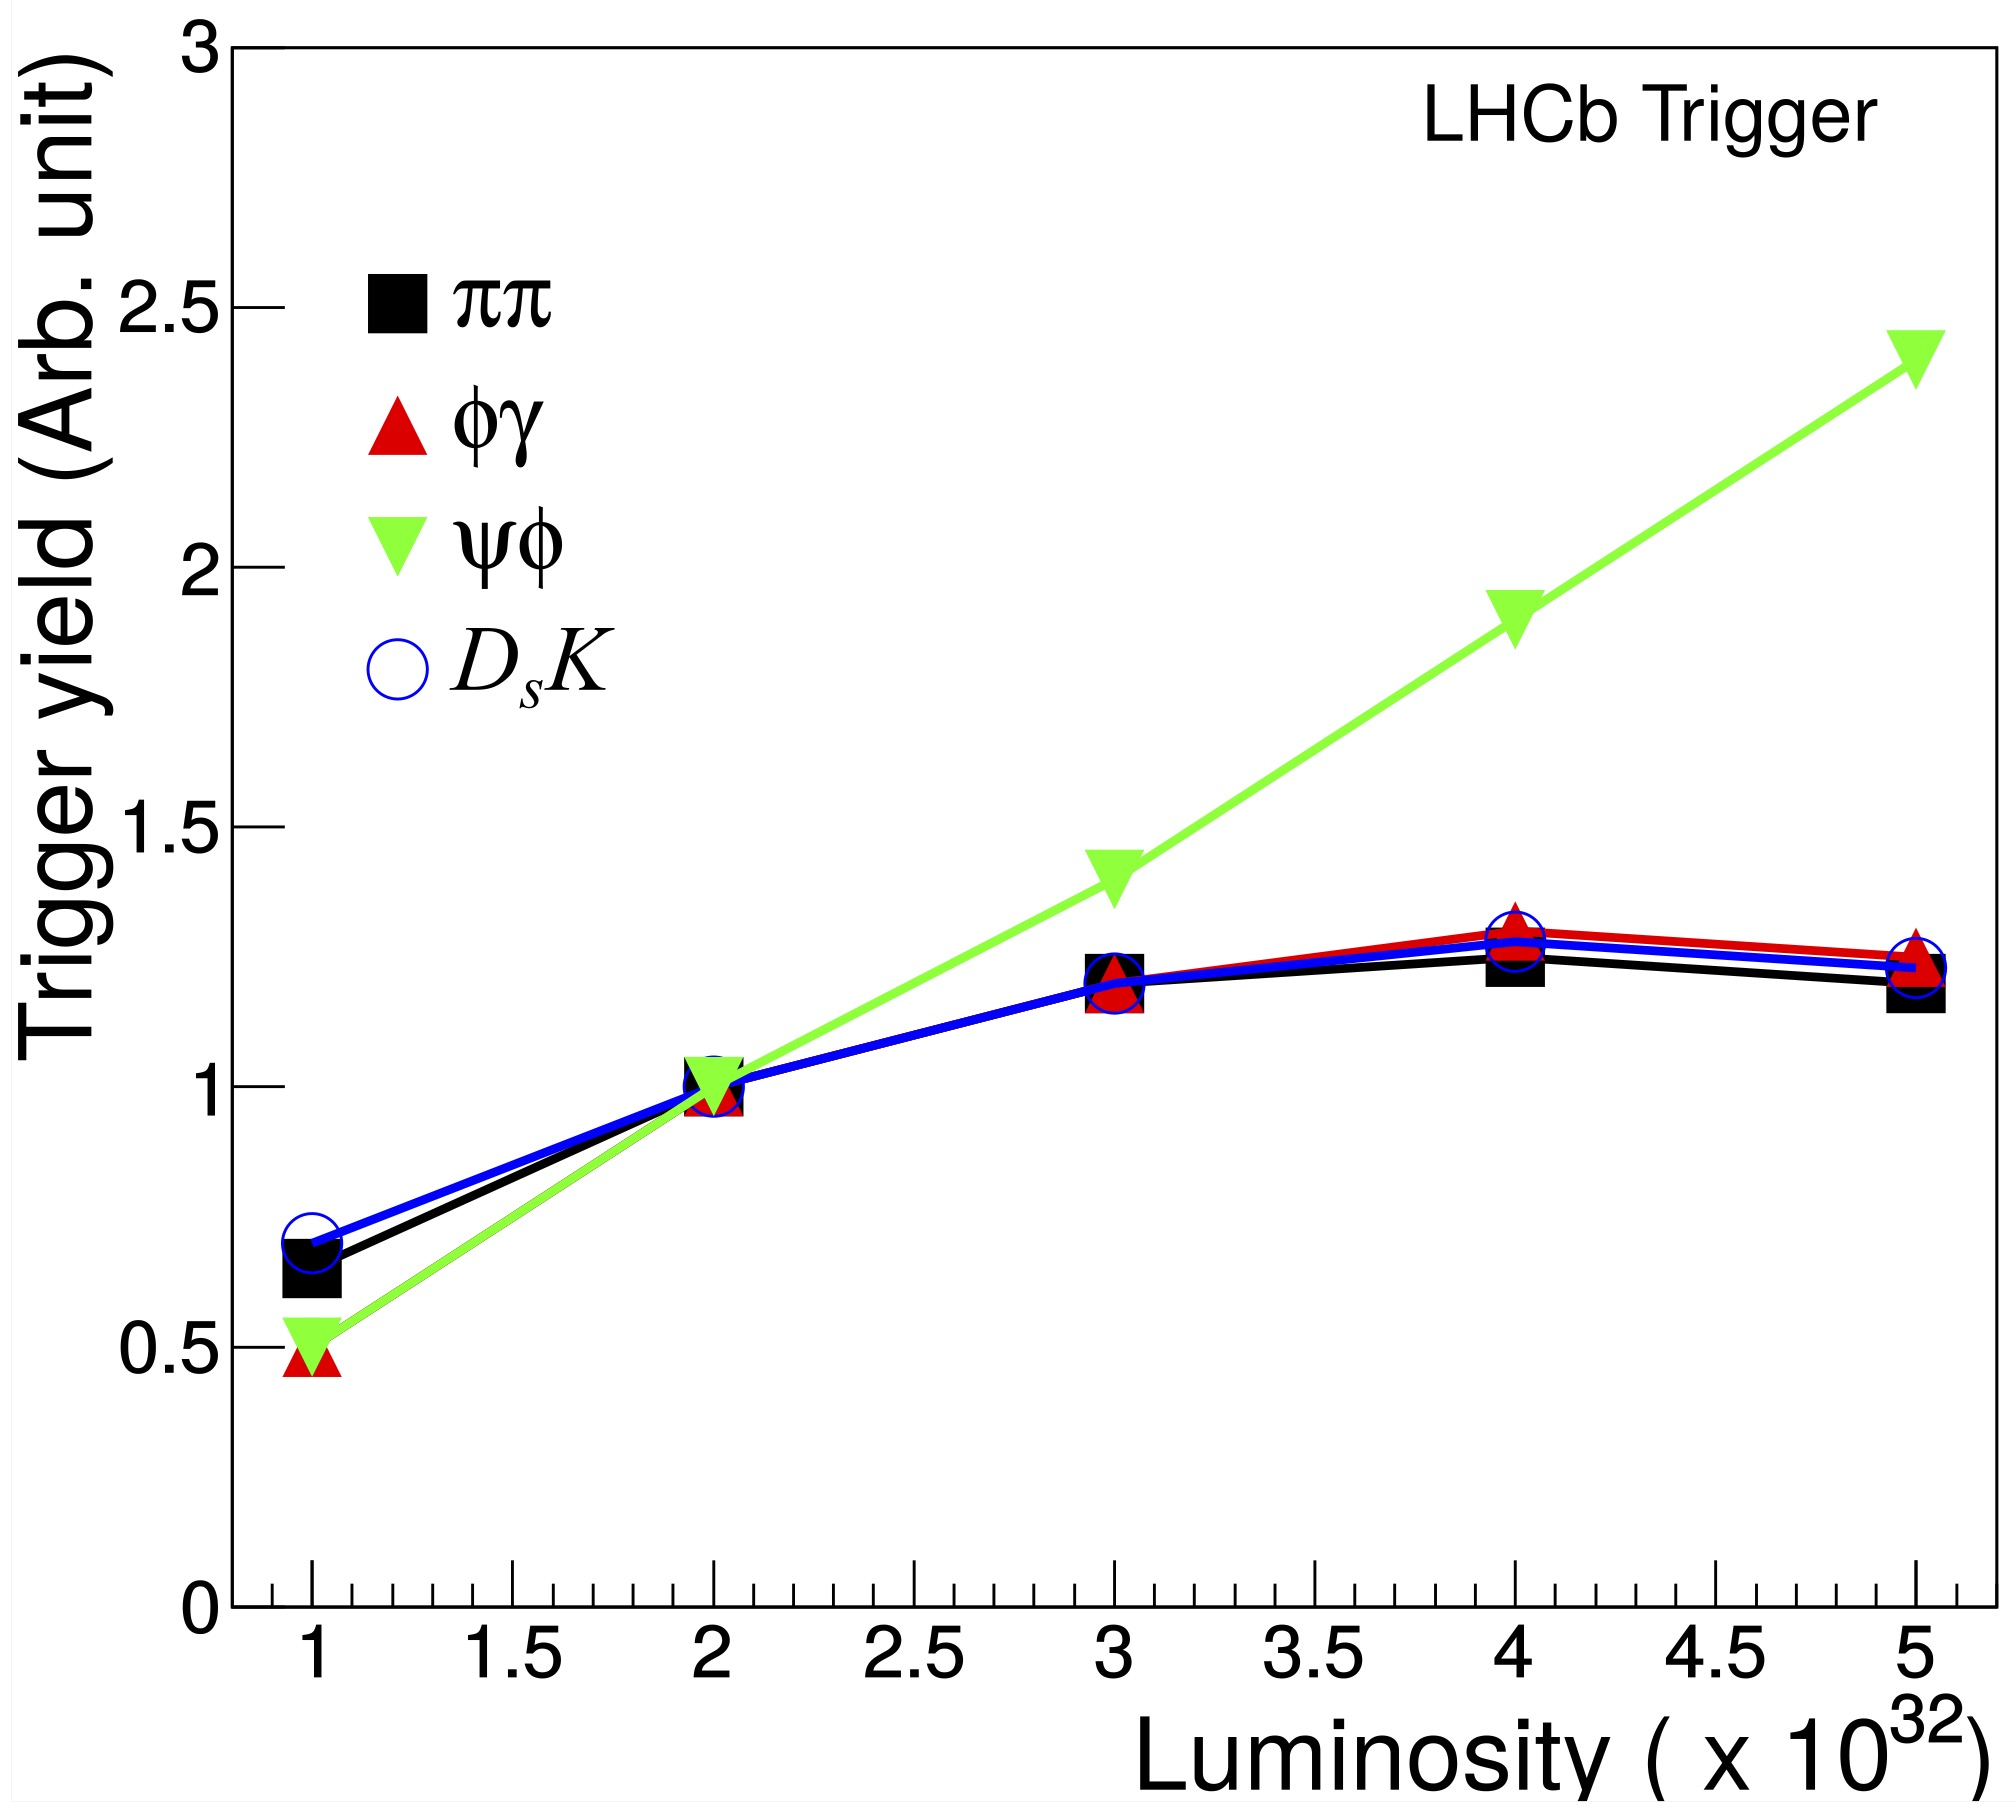
\includegraphics[width=\textwidth]{./dijkstra.png}
  \end{column}
  \begin{column}{.4\textwidth}
    \begin{alertblock}{what doesn't work}
    \begin{itemize}
        \item increased luminosity
        \item[$\rightarrow$] events passing hardware trigger
        \item[$\rightarrow$] saturating bandwidth
        \item[$\rightarrow$] tighten thresholds
        \item[$\rightarrow$] loss in efficiency
        \item[$\Rightarrow$] no increase in statistics for analyses
        \newline (depending on the decay channel)
    \end{itemize}
  \end{alertblock}
  \end{column}
  \end{columns}
  %data pile, dijkstra plot PID plot
\end{frame}

\begin{frame}
  \frametitle{removal of hardware trigger II}
  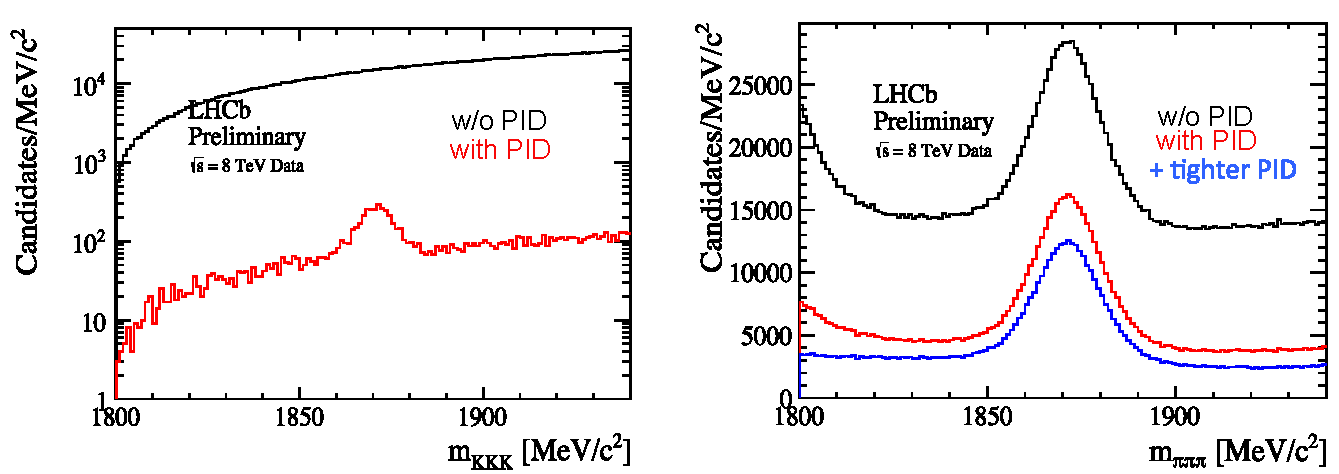
\includegraphics[width=\textwidth]{./stor.pdf}
  \begin{itemize}
      \item backgrounds from real physics events
      \item cannot distinguish signal from background w/o RICH PID
      \item[$\Rightarrow$] even selection in software
  \end{itemize}
\end{frame}

\begin{frame}[t]
  \frametitle{ }
  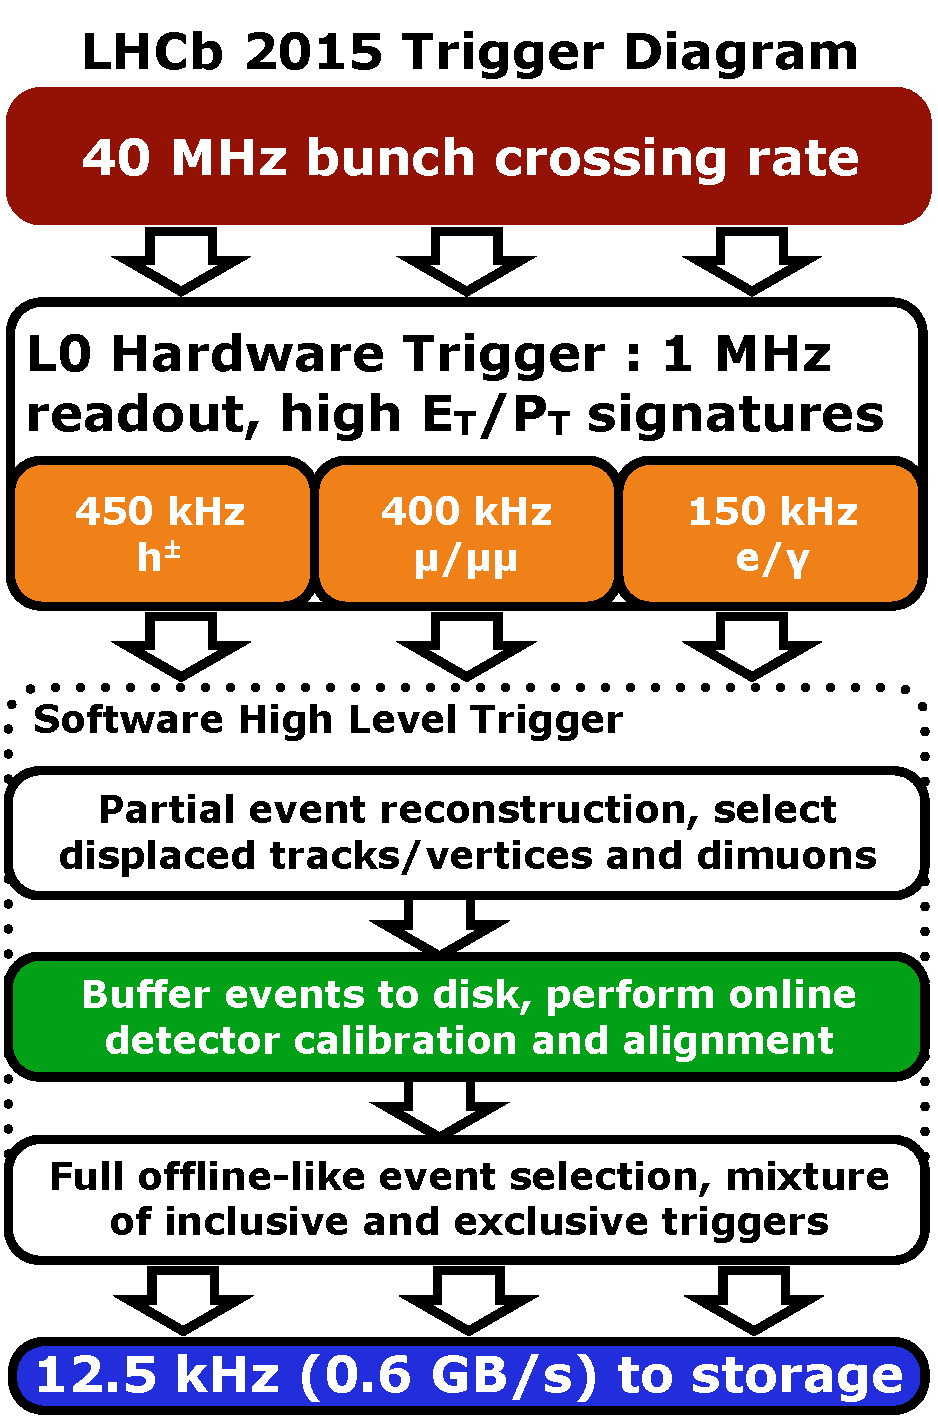
\includegraphics[width=.45\textwidth]{./LHCb_Trigger_RunII_May2015.pdf}
  \hspace{.01\textwidth}
  $\Rightarrow$
  \hspace{.01\textwidth}
  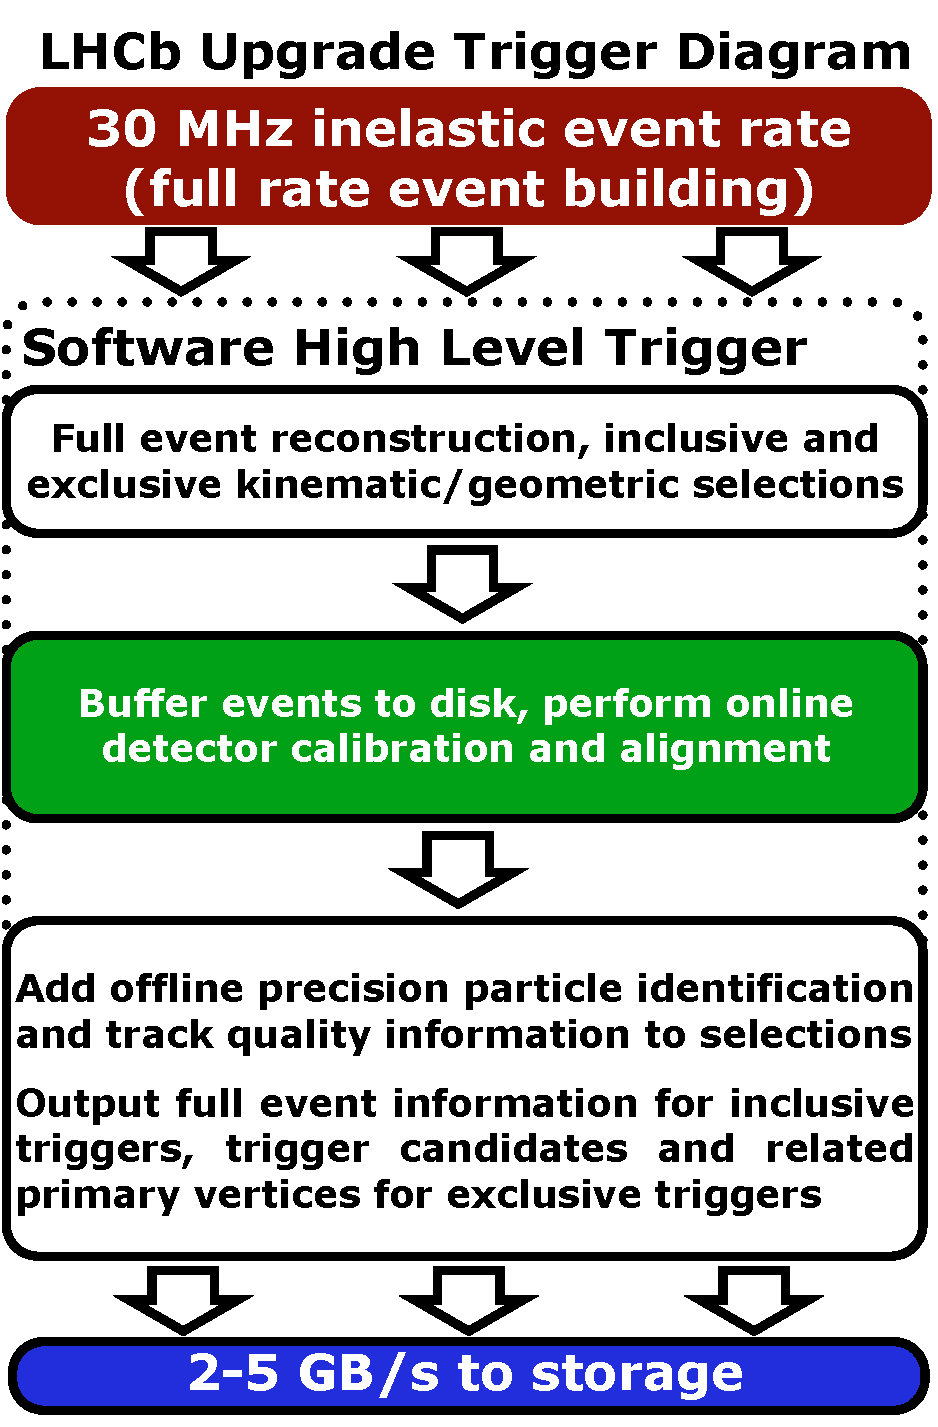
\includegraphics[width=.45\textwidth]{./LHCb_Trigger_RunIII_May2015.pdf}

  \vspace{-.9\textheight}
  \only<2>{
  {
    \begin{columns}
      \begin{column}{.5\textwidth}
    \end{column}
    \begin{column}{.5\textwidth}
      \begin{alertblock}{40 Tbit/s hardware readout}\end{alertblock}

      \vspace{.4\textheight}
      \begin{exampleblock}{relaxed latency}
        Calibration takes $\mathcal{O}$(minutes)

        Events stay buffered for $\mathcal{O}$(days)
      \end{exampleblock}
    \end{column}
    \end{columns}
  }
}
\end{frame}

\begin{frame}[t]
  \frametitle{Luxury problem: MHz signals}
  \begin{columns}\begin{column}{.6\textwidth}
  
\includegraphics[width=\textwidth]{./pile.pdf}
  \end{column}\begin{column}{.4\textwidth}
  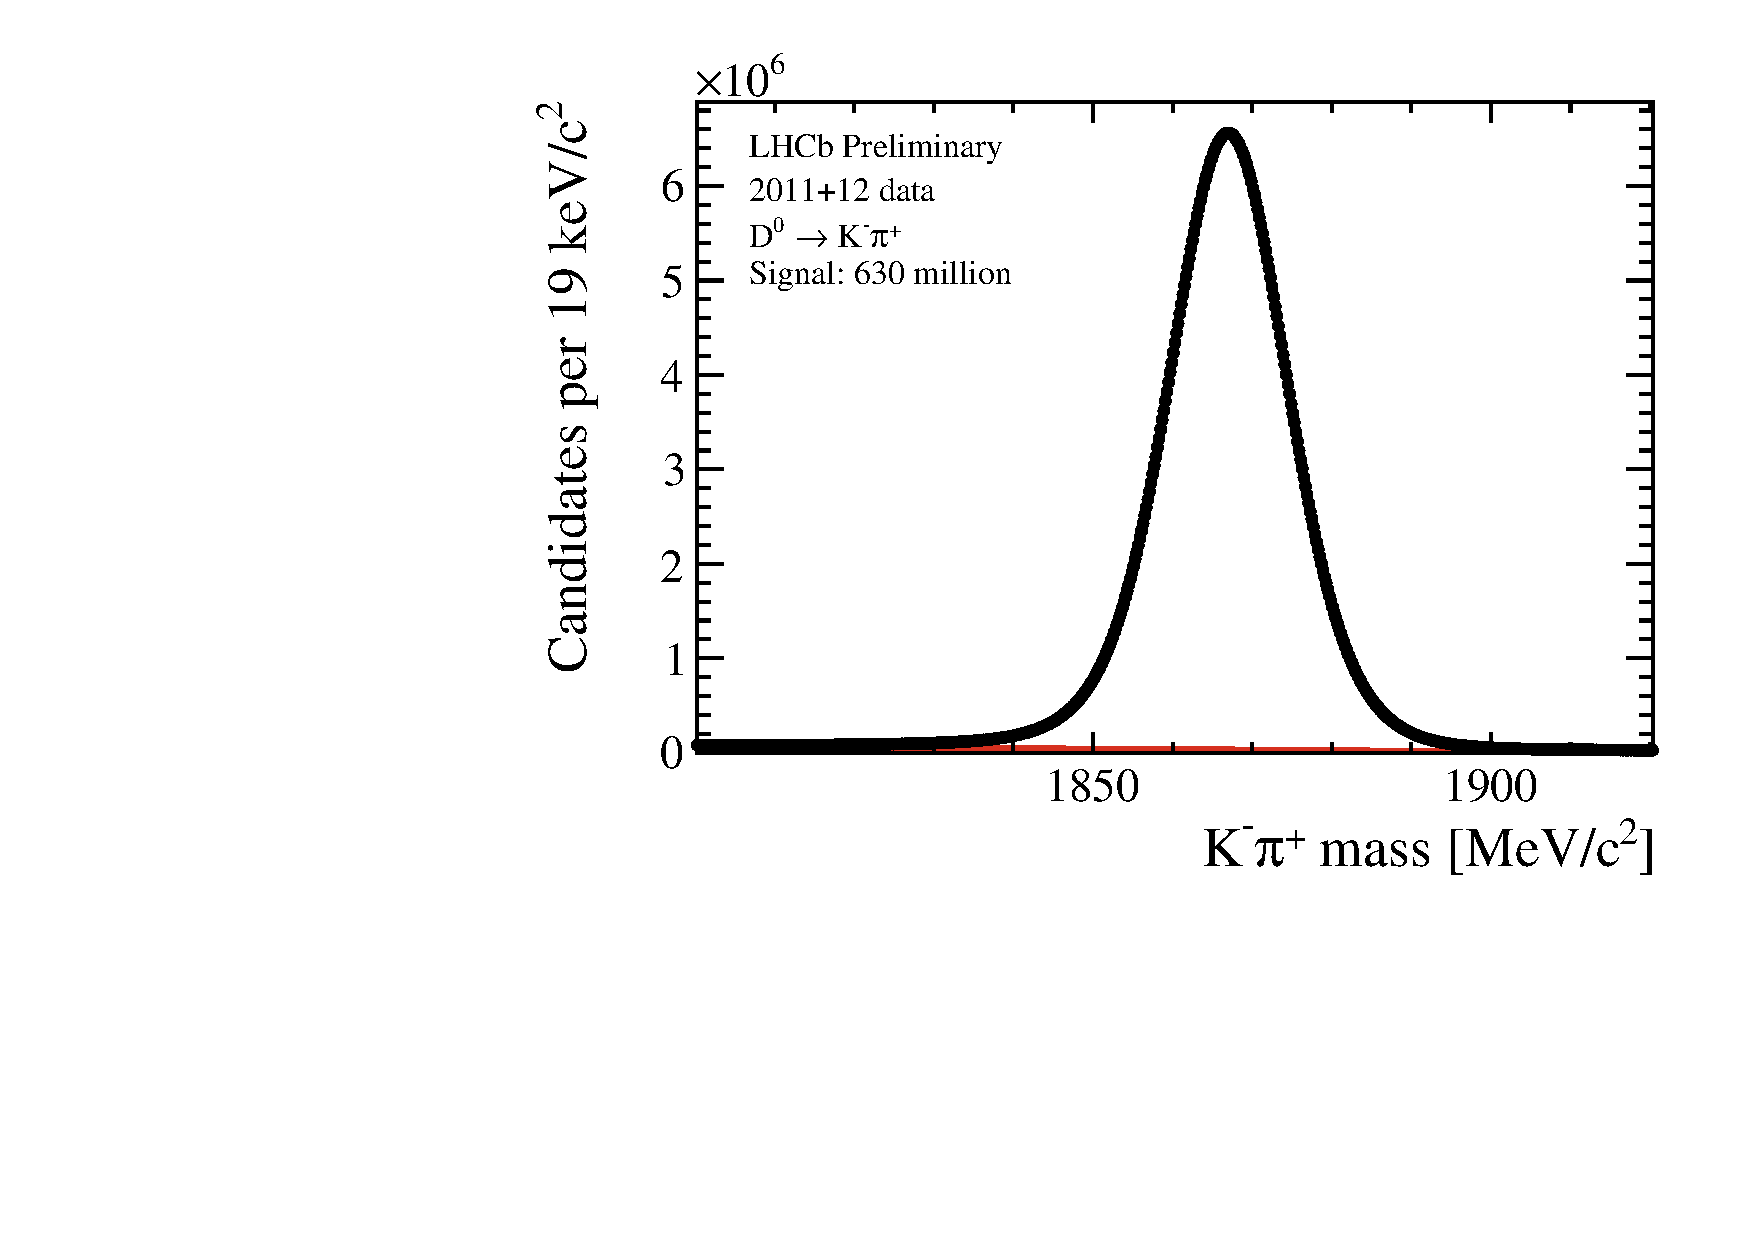
\includegraphics[height=\textwidth,angle =-90]{./Dmass.pdf}

  {~}\hspace{5em}\myhref{http://cds.cern.ch/record/2200233}{LHCb-CONF-2016-005}
\end{column}\end{columns}
  \only<1>{
  \begin{itemize}
    \item Selecting and storing full events could work for rare signal
    \item When dealing with ``millions'' of good signal events, rejecting background isn't enough to stay within processing bandwidths
  \end{itemize}
}
\only<2>{
  \begin{exampleblock}{The TURBO approach}
    \begin{itemize}
        \item once a decay is reconstructed (mass, decay time, Dalitz plot)
          \newline no need to access raw data for analysts
        \item once a decay is reconstructed in the trigger
          \newline no need to re-reconstruct offline

        \item (unaffordable to study raw data for millions of events anyway)
    \end{itemize}
  \end{exampleblock}
}
\only<3>{
  \begin{alertblock}{The TURBO approach}
    \begin{itemize}
        \item once a decay is reconstructed (mass, decay time, Dalitz plot)
          \newline \textcolor{red}{cannot afford} to store all raw data offline
        \item once a decay is reconstructed in the trigger
          \newline \textcolor{red}{cannot afford} to re-reconstruct all data offline

        \item \textcolor{red}{\textbf{Finite budget for offline computing resources}}
    \end{itemize}
  \end{alertblock}
}
\end{frame}

\begin{frame}
  \frametitle{store what you need}
  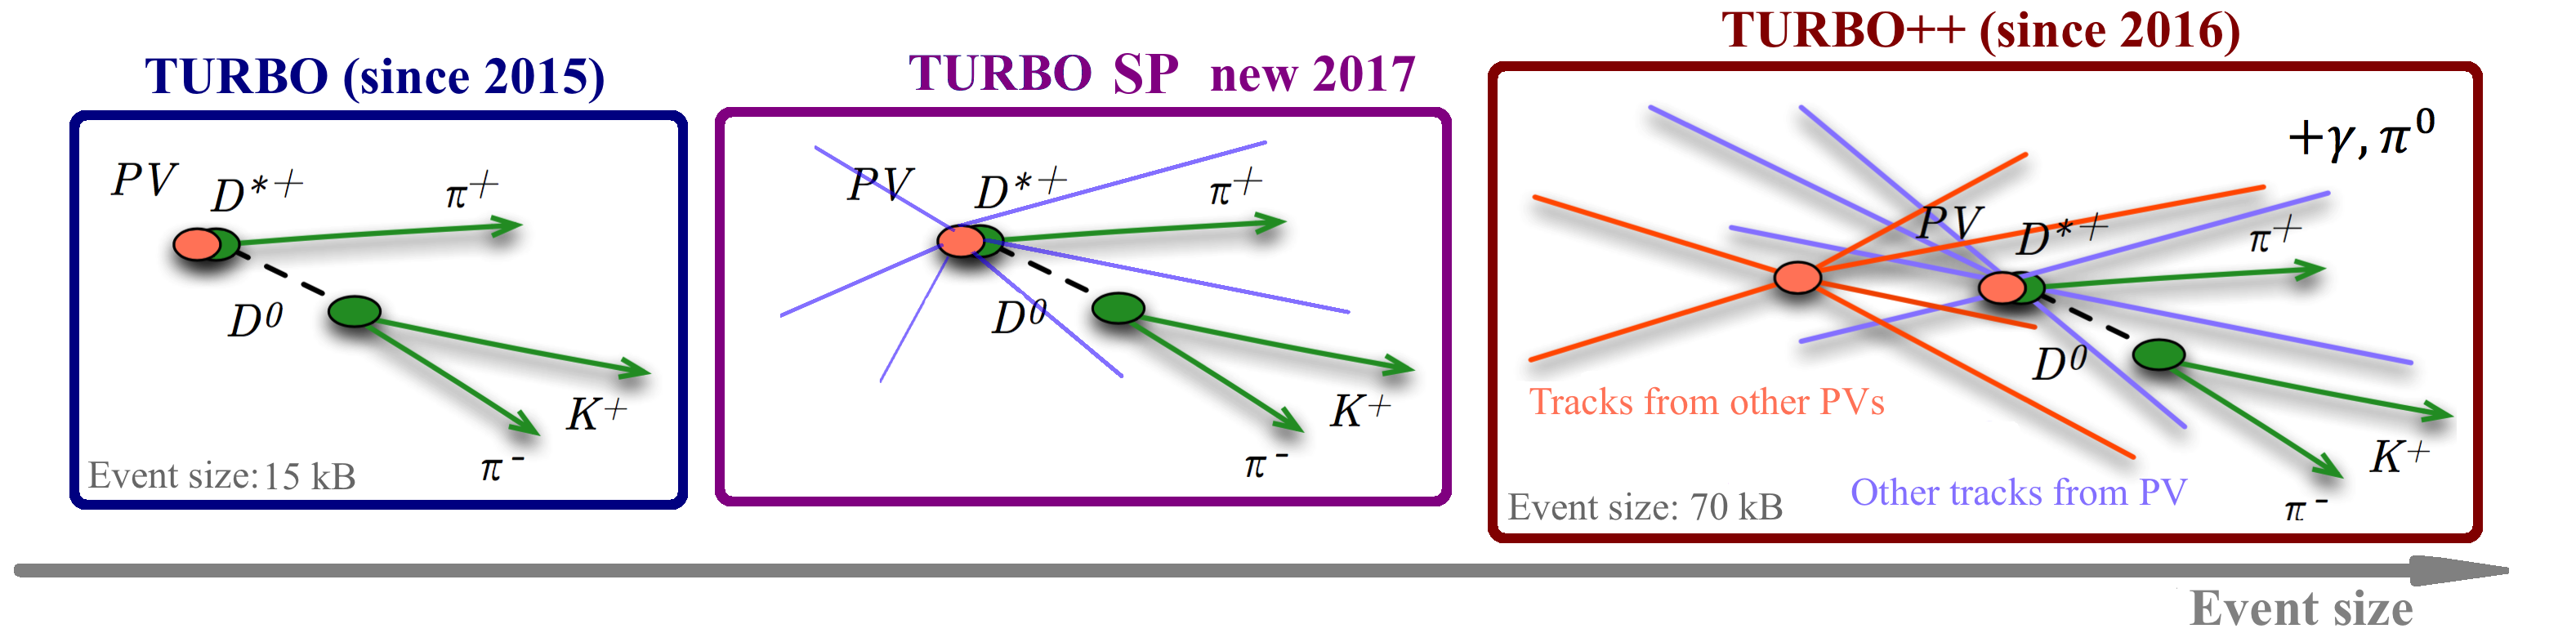
\includegraphics[width=\textwidth]{./turbosp.png}

  \myhref{http://dx.doi.org/10.1016/j.cpc.2016.07.022}{10.1016/j.cpc.2016.07.022}
  
  \begin{block}{per trigger line storage definition}
  \begin{itemize}
      \item only decay and nothing else
      \item decay and selected reconstructed objects
      \item all \emph{reconstructed} objects (no raw data)
      \item full raw event
  \end{itemize}
  TURBO triggers must be a default for many analyses
  \end{block}
\end{frame}

\begin{frame}
  \frametitle{Bandwidth division I}
  \begin{itemize}
    \item In a perfect world we could store and process all selected events
      \newline$\rightarrow$ we will face offline storage limits
    \item wide Physics program requires compromise
    \item limit \emph{sensitivity} loss in a fair share
  \end{itemize}

  \begin{block}{}
    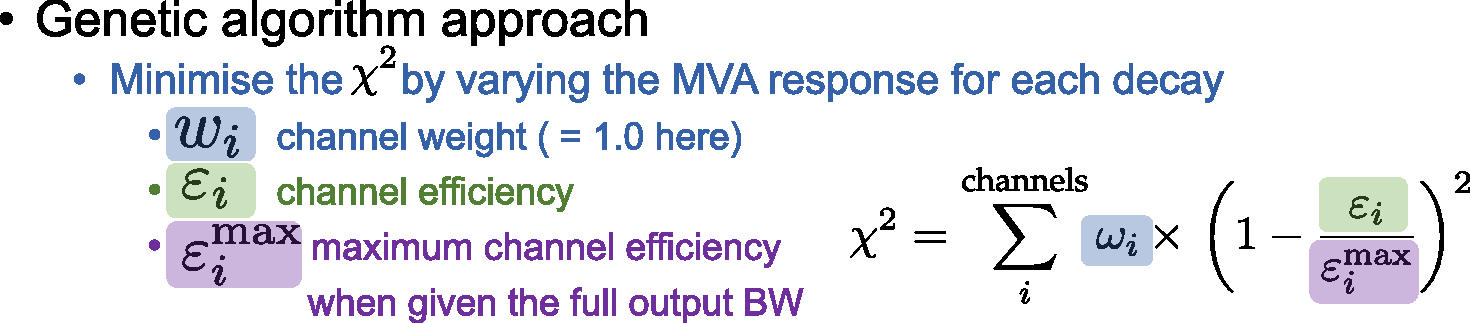
\includegraphics[width=\textwidth]{./BW.pdf}
    \begin{itemize}
        \item if sum of all channels exceeds total bandwidth \newline$\rightarrow$ assume random dropping of events
        \item weight to reduce impact of calibration channels\newline (different order of magnitude in branching fraction)
    \end{itemize}
  \end{block}

  \vspace{-1em}
  \myhref{https://cds.cern.ch/record/2244313}{LHCb-PUB-2017-006}
\end{frame}

\begin{frame}
  \frametitle{Bandwidth division II}
  \begin{columns}
    \begin{column}{.5\textwidth}
  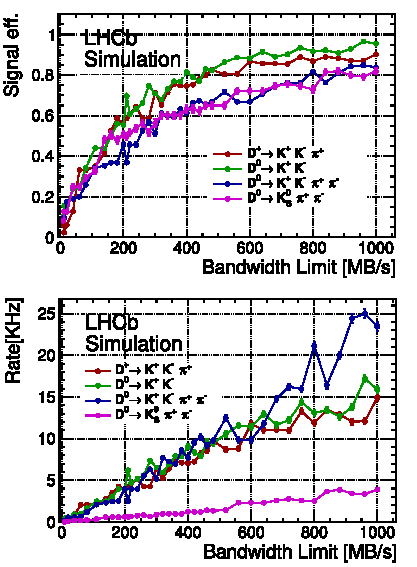
\includegraphics[width=\textwidth]{./BW-trend.pdf}
    \end{column}
    \begin{column}{.5\textwidth}
      going from maximal bandwidth to restricted bandwidth
      \begin{itemize}
      \item only small efficiency decrease
      \item ``90\,\% of the data holds 95\,\% of the statistical power''
      \item different persistency tested, too:\newline $D^0\to K_S\pi\pi$ as Turbo++\newline$\Rightarrow$ more restricted total rate
      \end{itemize}
    \end{column}
    \end{columns}
  \end{frame}

\begin{frame}
  \frametitle{``Moore doesn't obey Moore's law''}

  \begin{columns}
    \begin{column}{.5\textwidth}
      \begin{overpic}[width=\textwidth]{./moore.png}
        \put (15,50) {\tiny{\textrm{LHCb computing}}}
      \end{overpic}
    \end{column}
    \begin{column}{.5\textwidth}

  \begin{itemize}
    \item theoretical computing power of CPUs increases (per second, per Watt, per CHF)
    \item observed computed trigger decisions does not follow that increase
  \end{itemize}
    \end{column}
    \end{columns}
    \begin{alertblock}{reasons from a CPU's point of view \only<2>{II}\only<1>{I}/II}
    \only<1>{
  \begin{itemize}
    \item modern vector units process 2, 4, or 8 inputs at a time
      \newline$\leadsto$ our software often didn't use these
      \newline$\rightarrow$ 7/8 of the silicon unused!
  \end{itemize}
    }
    \only<2>{
  \begin{itemize}
    \item software not parallelised (just start multiple processes on a multicore machine)
    \newline$\leadsto$ processes compete for memory
    \newline$\leadsto$ even multiple instances of the same data (detector geometry)
    \newline$\rightarrow$ CPU waits for data instead of computing
  \end{itemize}
    }
\end{alertblock}

\end{frame}

\begin{frame}
  \frametitle{tracking sequence}
  \begin{columns}
    \begin{column}{.5\textwidth}
      \myhref{https://cds.cern.ch/record/2244312}{LHCb-PUB-2017-005}

      \only<1>{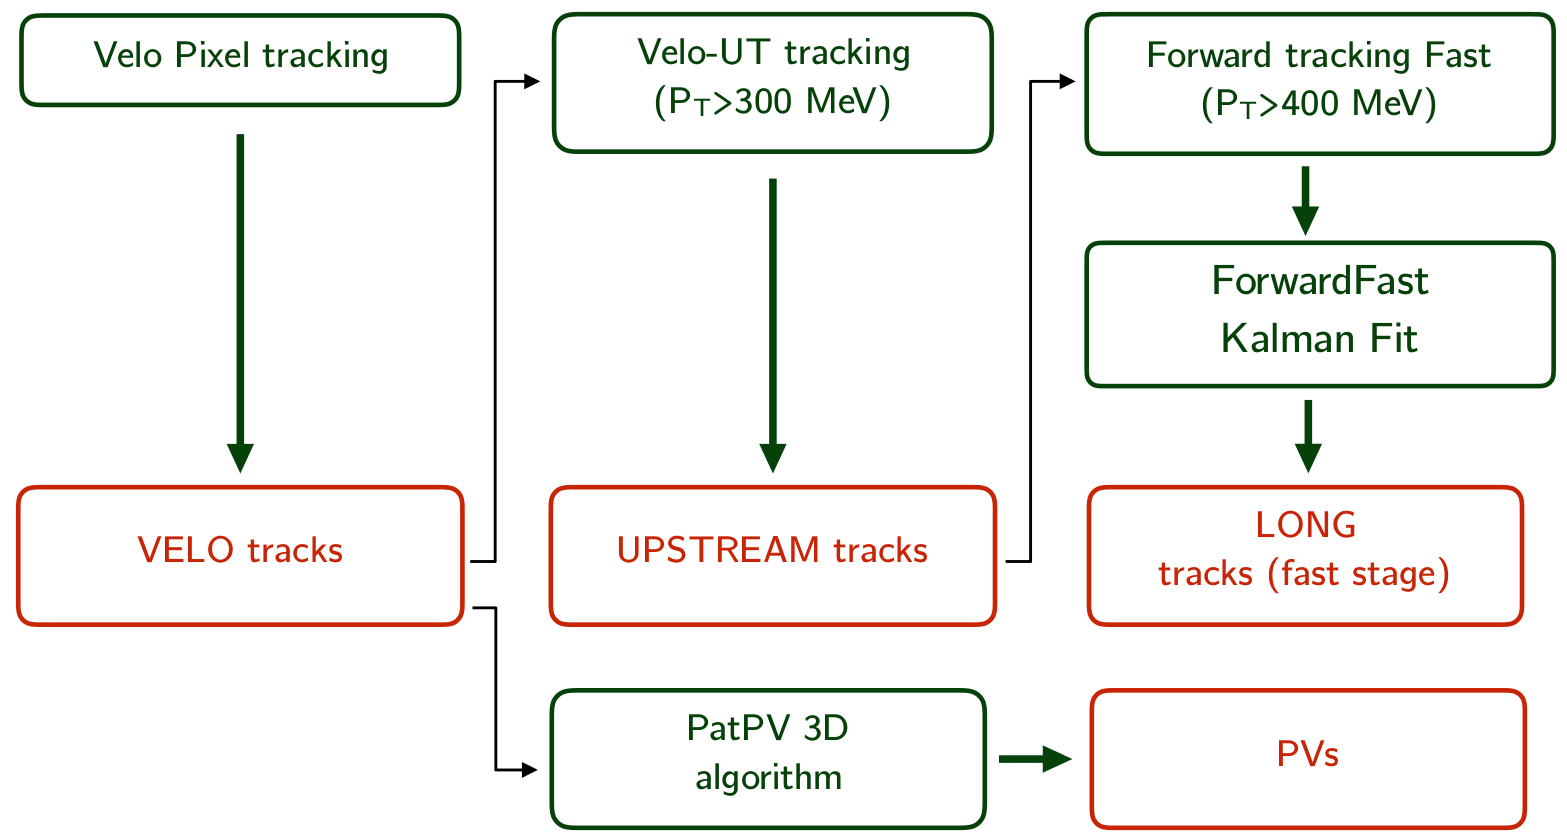
\includegraphics[width=\textwidth]{./fast.png}
    
      fast sequence $\unit{6.0}{ms/evt}$ @ \unit{30}{MHz}
      {\small{
        \begin{tabular}{ll}
          VELO tracking    & $\unit{2.0}{ms/evt}$  \\
          VELO-UT tracking & $\unit{0.5}{ms/evt}$  \\
          forward tracking & $\unit{2.3}{ms/evt}$  \\
          PV finding       & $\unit{1.1}{ms/evt}$  \\
        \end{tabular}
      }}

      (present HLT1: $\unit{35}{ms}$)
    
    }
      \only<2>{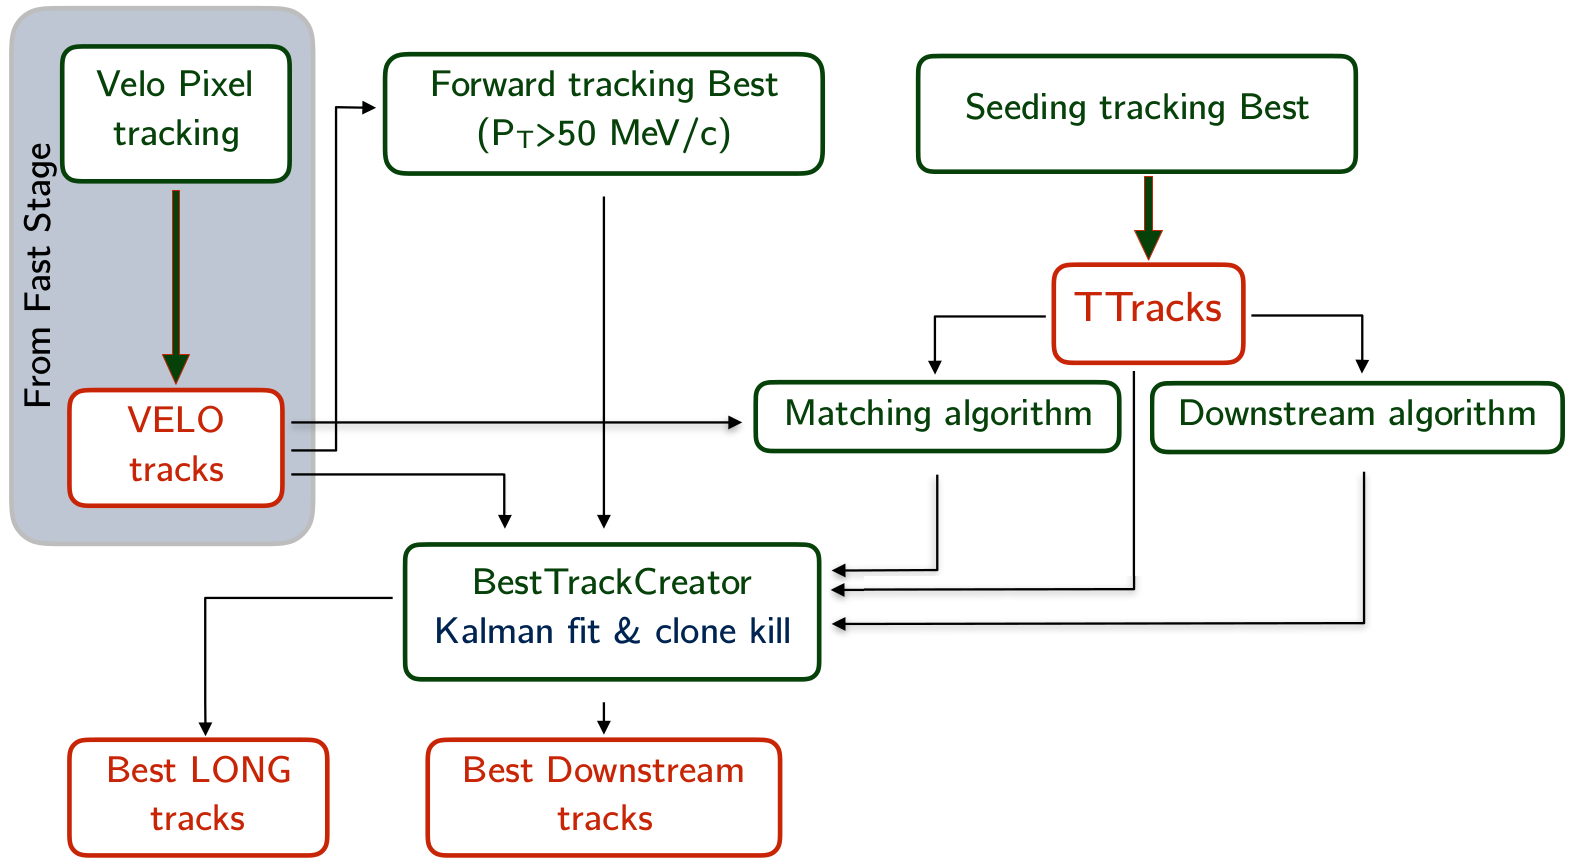
\includegraphics[width=\textwidth]{./full.png}
    
%      $\unit{6.0}{ms/evt}$
%      \begin{itemize}
%        \item[VELO tracking] $\unit{2.0}{ms/evt}$
%        \item[VELO-UT tracking] $\unit{0.5}{ms/evt}$
%        \item[forward tracking] $\unit{2.3}{ms/evt}$
%        \item[PV finding] $\unit{1.1}{ms/evt}$
%      \end{itemize}

      %fast sequence $\unit{6.0}{ms/evt}$ @ $\unit{30}{MHz}$
      full sequence aim
      {\small{\begin{tabular}{l}
        $\sim 20\times$ slower\\ $1/30$ rate (\unit{1}{MHz})\end{tabular}}}
      \newline Kalman fit large contributor
      \newline (present HLT2: $\unit{650}{ms}$)
    }
    
  \end{column}
  \begin{column}{.5\textwidth}
    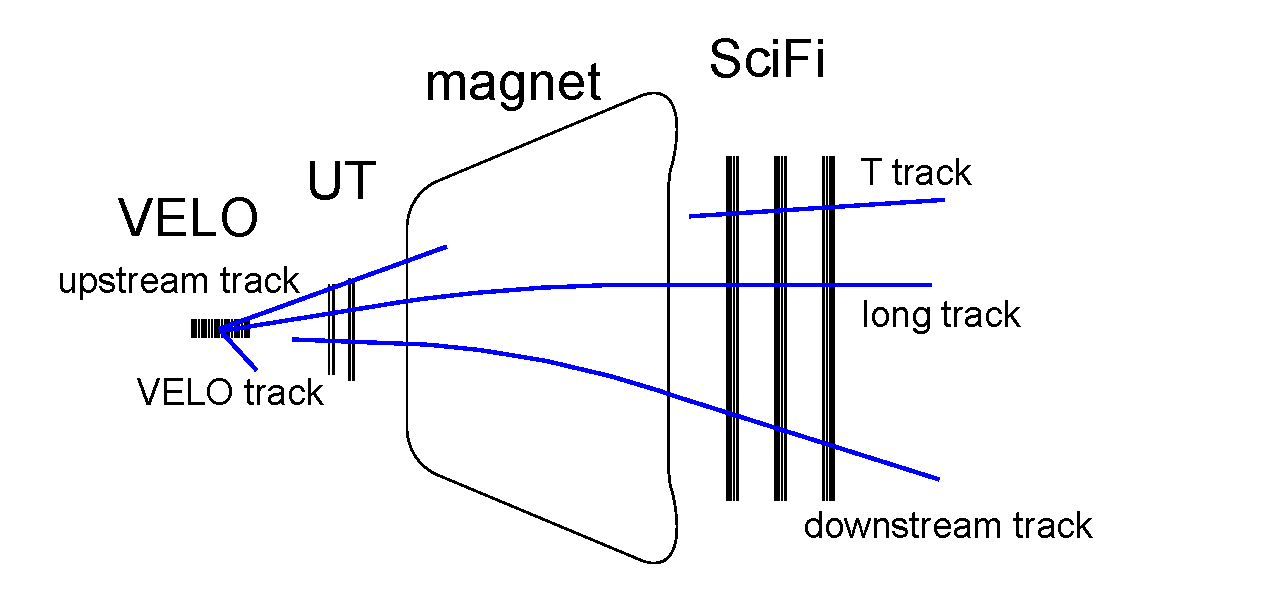
\includegraphics[width=.8\textwidth]{./ttypes.pdf}
    \begin{itemize}
        \item similar to current software trigger
          \item single track and two track selections for displaced objects
            \newline (``easy'' combinatorics, limited reconstruction)
            \item<2-> reconstruct remaining tracks in the ``full stage''
              \item<2-> also reconstruct decay products of strange decays outside the VELO
    \end{itemize}
  \end{column}
  \end{columns}
\end{frame}

\begin{frame}
  \frametitle{Kalman filter track fit}
  \only<1>{
  \begin{itemize}
      \item track fit one of the big CPU time consumers
        \item written for sequential adding of hits
        \item but different tracks can be fitted independent of each other
          \newline (thread parallelisable)
        \item matrix operations are always the same
          \newline (vectorisable)
  \end{itemize}
}
\only<2>{
  \begin{alertblock}{grain of salt}
    \begin{itemize}
        \item only speeds up the matrix algebra
        \item material lookup remains
        \item now requires back-and-forth conversion of memory layout
        \item[$\Rightarrow$] to be consequent need to adapt underlying event model
    \end{itemize}
  \end{alertblock}
}
  \begin{columns}
    \begin{column}{.5\textwidth}
  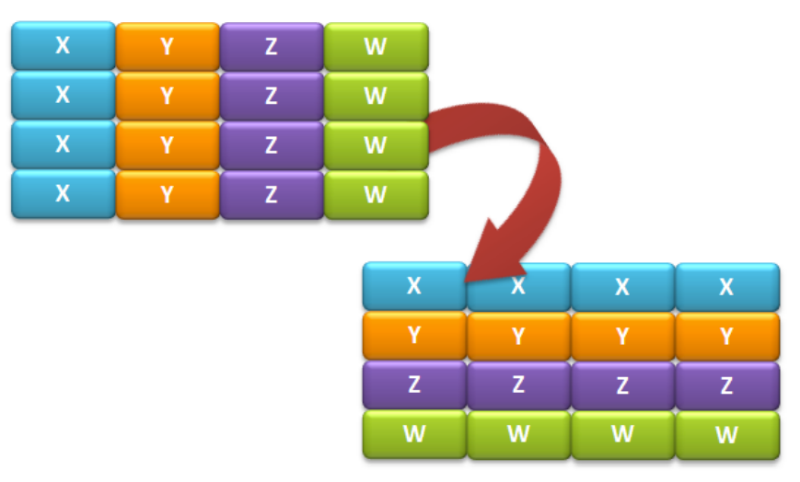
\includegraphics[width=\textwidth]{./SIMD.pdf.png}
    \end{column}
    \begin{column}{.5\textwidth}
      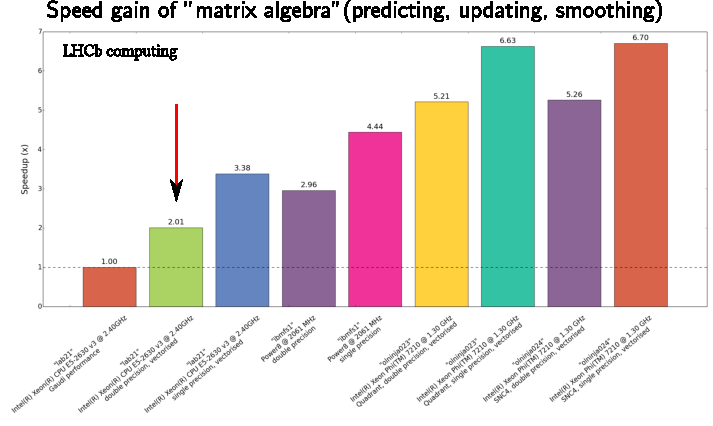
\includegraphics[width=\textwidth]{./kalspeed.pdf}
    \end{column}
    \end{columns}
    \myhref{https://cds.cern.ch/record/2229971}{LHCb-TALK-2016-372}
\end{frame}

\begin{frame}[t]
  \frametitle{parametrised Kalman fit}
  \begin{itemize}
    \item avoid first-principles math for every track
      \newline $\leadsto$ parametrisations can be equally accurate
      \newline reduce complicated $B$ field propagation and material lookup to $\mathcal{O}(20)$ parameters
  \end{itemize}
  \only<1>{\begin{block}{example parametrised extrapolation through the magnet}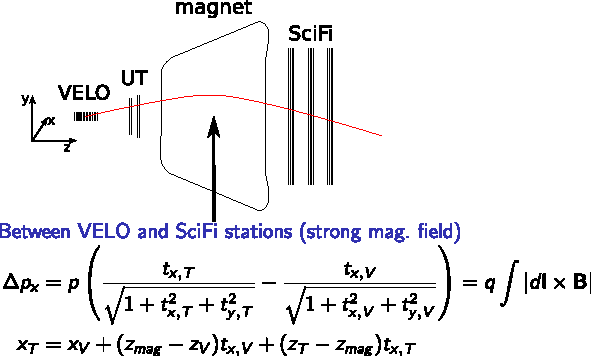
\includegraphics[width=.6\textwidth]{./parametrisation.pdf}

  \myhref{https://cds.cern.ch/record/2255840}{LHCb-TALK-2017-047}
\end{block}
}
  \only<2->{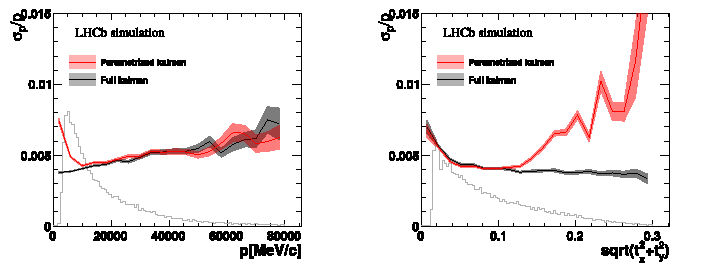
\includegraphics[width=\textwidth]{./param.pdf}}
  \only<3->{
    \vspace{-.4\textheight}
  \begin{exampleblock}{work in progress}
    \begin{itemize}
        \item resolution close to reference
        \item potentially use full fit for tracks with large $\sqrt{t_x^2+t_y^2}$
        \item find alternative parametrisations
        \item[$\Rightarrow$] fast track fit must not deteriorate resolution
    \end{itemize}
  \end{exampleblock}
}
\end{frame}

\begin{frame}
  \frametitle{fake track identification}
  \begin{itemize}
      \item fake tracks a big contribution to computing budget in run~I
      \item identification of fakes w/ neural network after track fit more powerful than track fit $\chi^2$ alone
      \item<2-> As more and more ML goes into earlier stages of the track reconstruction, there are less fakes to remove after the track fit
      \item[$\rightarrow$]<2-> looking forward for this to become less important
  \end{itemize}
  \begin{columns}
    \begin{column}{.5\textwidth}
      upgrade fake rejection:

  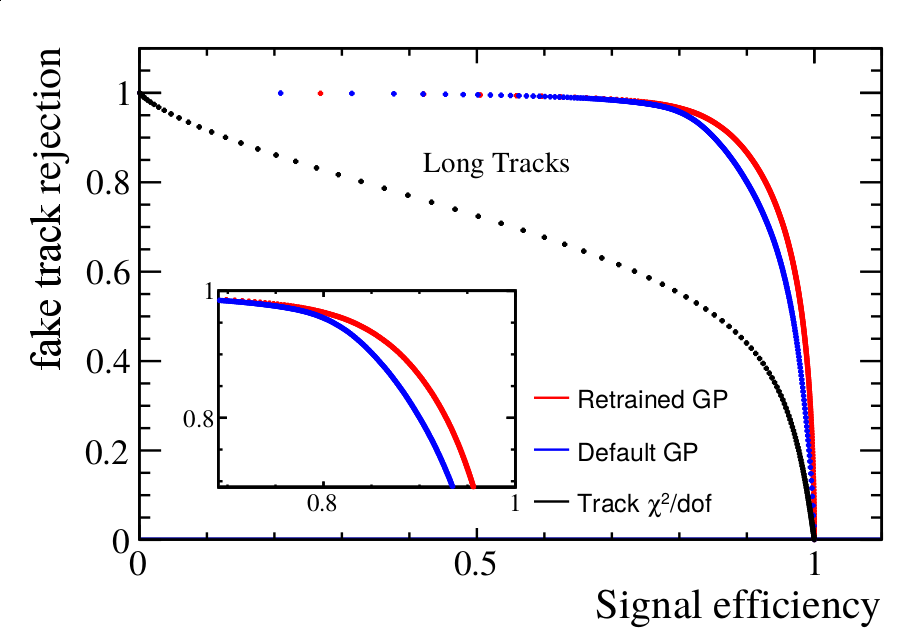
\includegraphics[width=\textwidth]{./GPlong.png}
\end{column}
    \begin{column}{.5\textwidth}
      \begin{exampleblock}{impact on run II}
        \begin{itemize}
          \item RICH PID $- \mathcal{O}(20\,\%)$ CPU
            \item combinatorics $- \mathcal{O}(60\,\%)$ CPU
            \item trigger $- \mathcal{O}(30\,\%)$ rate
        \end{itemize}
      \end{exampleblock}
\end{column}
\end{columns}

\end{frame}

\begin{frame}
  \frametitle{multi threaded processing framework}
  \begin{columns}
    \begin{column}{.45\textwidth}
      \begin{overpic}[width=\textwidth]{./thread.pdf}
        \put (10,90) {\tiny{\textrm{LHCb computing}}}
        \put (10,35) {\tiny{\textrm{LHCb computing}}}
      \end{overpic}
      %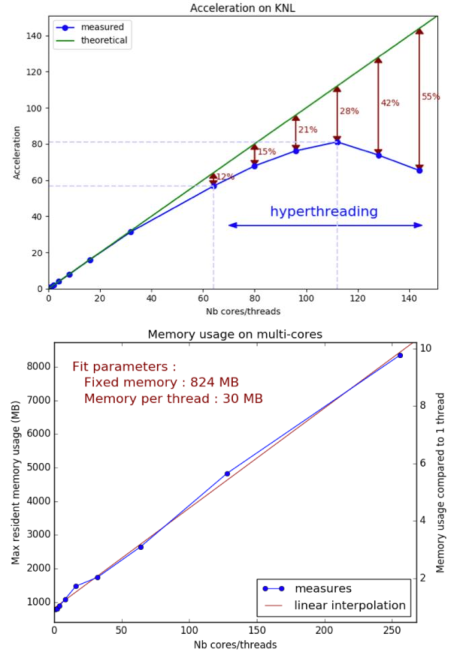
\includegraphics[width=\textwidth]{./thread.pdf}
    \end{column}
    \begin{column}{.55\textwidth}
      \begin{itemize}
        \item introduce harder framework constrains
            \newline (functional programming)
            \item observe near optimal speedup when increasing number of threads
            \item observe little memory increase when increasing number of threads
      \end{itemize}
    \end{column}
    \end{columns}
\end{frame}


\begin{frame}
  \frametitle{Conclusion}
  \begin{itemize}
    \item LHCb physics program relies on software trigger at $\unit{30}{MHz}$
    \item Need to face tight constraints from offline storage and processing
      \newline as well as online processing power
      \begin{itemize}
        \item[$\rightarrow$] reconstruction right out of the trigger
        \item[$\rightarrow$] ``per analysis'' storage 
      \end{itemize}
    \item Fast tracking \emph{without performance loss} crucial for LHCb upgrade
      \item Needs reconstruction software close to computer hardware to optimally use it
  \end{itemize}

\end{frame}

\appendix

    \beamertemplateshadingbackground{blue!80!black}{Black}


\begin{frame}
  \begin{center}
    \textcolor{bandgreen}{\Huge{\textsc{backup}}}
  \end{center}
\end{frame}

    \beamertemplateshadingbackground{white!10!white}{White}

\begin{frame}
  \frametitle{these slides online}
  
\includegraphics[width=.5\textwidth]{./qr.eps}

  \myhref{https://gitlab.cern.ch/pseyfert/Vertex2017}{https://gitlab.cern.ch/pseyfert/Vertex2017}
\end{frame}

\begin{frame}
  \frametitle{parametrisations I}
  \begin{columns}\begin{column}{.5\textwidth}
      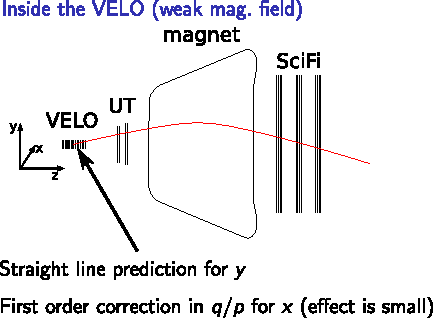
\includegraphics[width=\textwidth]{./paravelo.pdf}
  \end{column}\begin{column}{.5\textwidth}
      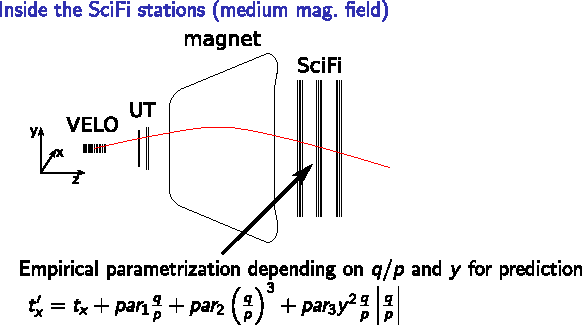
\includegraphics[width=\textwidth]{./paratstat.pdf}
  \end{column}\end{columns}
  \myhref{https://cds.cern.ch/record/2255840}{LHCb-TALK-2017-047}
\end{frame}\begin{frame}
  \frametitle{parametrisations II}
  \begin{columns}\begin{column}{.7\textwidth}
      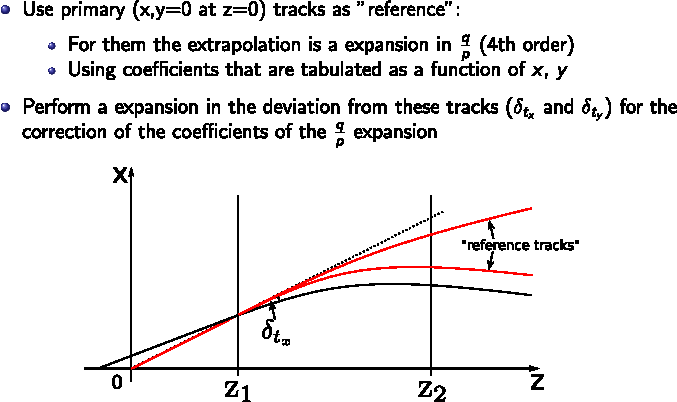
\includegraphics[width=\textwidth]{./deltatx.pdf}
  \end{column}\end{columns}
  \myhref{https://cds.cern.ch/record/2255840}{LHCb-TALK-2017-047}
\end{frame}

\begin{frame}
  \frametitle{Vertex resolution}
  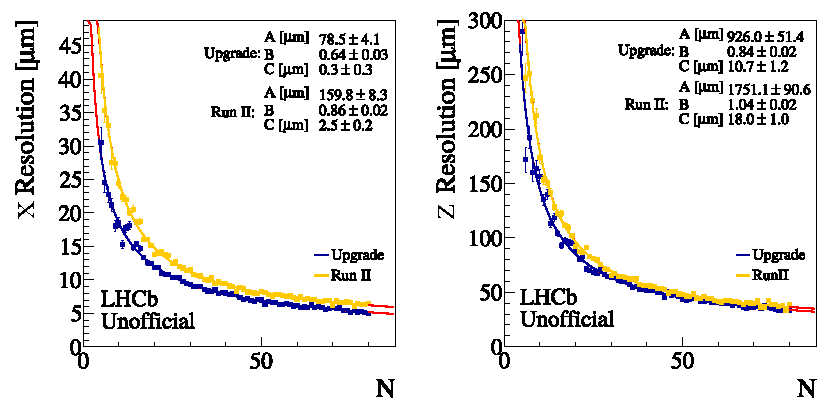
\includegraphics[width=\textwidth]{./vertexresolution.pdf}

      \myhref{https://cds.cern.ch/record/2244312}{LHCb-PUB-2017-005}
\end{frame}

    \begin{frame}
      \frametitle{Upgrade of the tracking system}
      \begin{columns}
        \begin{column}{.6\textwidth}
          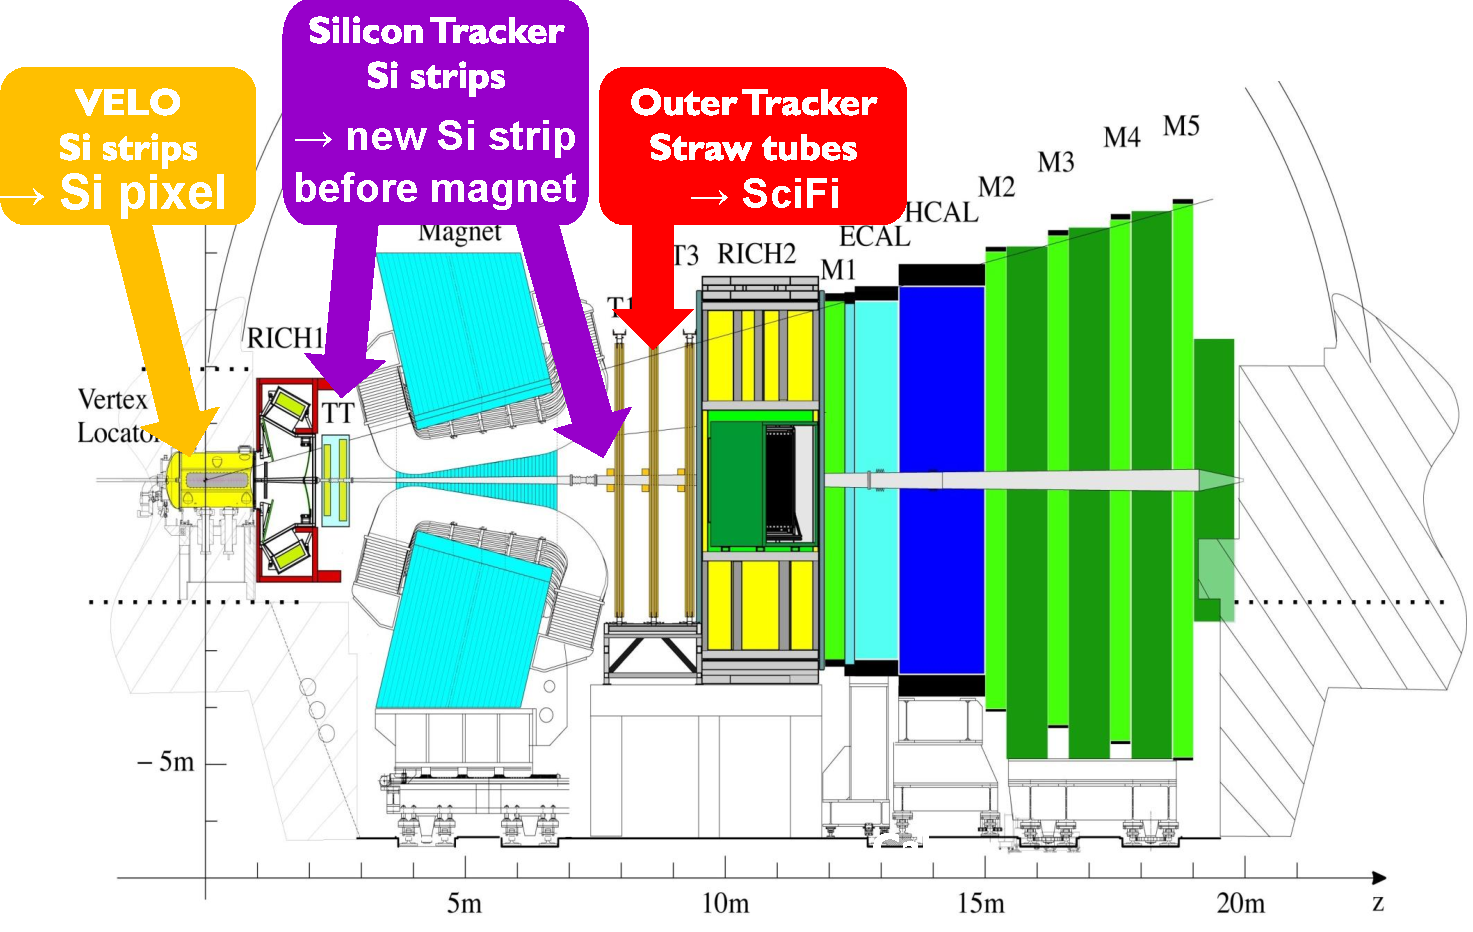
\includegraphics[width=\textwidth]{./LHCb2.pdf}
        \end{column}
        \begin{column}{.4\textwidth}
            \begin{itemize}
              \item Vertex pixel detector
                \newline see talk by Edgar Lemos Cid
              \item silicon strip detector
                \newline see talk by Marco Petruzzo
              \item scintilating fiber tracker
            \end{itemize}
          \end{column}
        \end{columns}
        \begin{columns}
        \begin{column}{.8\textwidth}
          \begin{block}{$\sigma_t$ (decay)}
            {\textcolor{white}{
            $<\unit{45}{\femto\second}$
            \newline $\left(\mathcal{D}\sim \exp(-\underbrace{\Delta m^2}_{1/\unit{56}{\femto\second}}\sigma_t^2/2)\right)$
            \newline for time dependent $B_s$ analyses
          }}
          \end{block}
          \end{column}
        \end{columns}
      \end{frame}

\end{document}
